\documentclass{article}
\usepackage{graphicx}
\usepackage[margin=1in]{geometry}
\usepackage[outdir=./]{epstopdf}  					% Avoids errors when input figures
\usepackage[labelsep=period,labelfont=bf]{caption}
%\usepackage{subcaption}

\begin{document}
	\begin{figure}[tbph]
		\caption{Comovement of the 10-Year Yields} \label{fig:dy_rolling_10y_nomsyn}
		\begin{center}
			\begin{minipage}{0.9\linewidth}
				\begin{center}
					\begin{subfigure}[t]{\linewidth}
						\includegraphics[trim={0cm 0cm 0cm 0cm},clip,height=0.38\textheight,width=\linewidth]{../Figures/Estimation/rolling10y_nomsyn.eps} \\
						\vspace{-0.37cm}
						\caption{Rolling Correlations} \label{subfig:rollingTSEM}
%						\vspace{0.4cm}
					\end{subfigure}
					
					\begin{subfigure}[t]{\linewidth}
						\includegraphics[trim={0cm 0cm 0cm 0cm},clip,height=0.38\textheight,width=\linewidth]{../Figures/Estimation/dy_index10y_nomsyn.eps} \\
						\vspace{-0.37cm}
						\caption{Connectedness Index} \label{subfig:dyindexTSEM}
						\vspace{0.2cm}
					\end{subfigure}
				
				\end{center}
				\vspace{-0.45cm}
				\fignotes{This figure plots rolling window correlation coefficients and the \cite{DieboldYilmaz:2014} connected index for the nominal yields of emerging markets and advanced countries, and the synthetic yields of emerging markets.The first panel displays one-year rolling correlations of daily yield changes averaged across all country pairs. The connected index in the second panel is obtained using a vector autoregression of order 1 of daily yield changes, with a forecast horizon of 10 days and a rolling window of 150 days.}
			\end{minipage}
		\end{center}
	\end{figure}
\end{document}
% trim = {<left> <lower> <right> <upper>}